% Slides — Capítulo 6: Nuvens
\documentclass[aspectratio=169,11pt]{beamer}
\usepackage{../comum/temameteo}
\graphicspath{{../figuras/cap06/}}

\title[Cap. 6 --- Nuvens]{Capítulo 6 --- Nuvens}
\subtitle{Meteorologia Prática}
\author{}
\date{}

\begin{document}

\begin{frame}
  \titlepage
  \vfill
  \atribuicao
\end{frame}

\begin{frame}{Roteiro}
  \tableofcontents
\end{frame}

% ---------------------------------------------------------------
\section{Classificação}

\begin{frame}{Os 10 gêneros em um desenho}
  \begin{columns}
    \column{0.4\textwidth}
    \begin{itemize}
      \item \emph{cirro-} alto $\cdot$ \emph{alto-} médio $\cdot$
            \emph{nimbo-} chuva $\cdot$ \emph{strato-} camada $\cdot$
            \emph{cumulo-} bolha.
      \item Estratiformes: ar estável levantado devagar (frentes,
            Cap.~12).
      \item Cumuliformes: convecção (Cap.~5 decide).
      \item Altas $=$ gelo: halos, cara fibrosa (Cap.~4: $e_s$ do
            gelo).
    \end{itemize}
    \column{0.6\textwidth}
    \figlivroslide{fig_06_5b.jpg}{0.58\textheight}{Fig.~6.5 --- gêneros
      por altura, aparência e composição}
  \end{columns}
\end{frame}

\begin{frame}{A família convectiva}
  \begin{columns}
    \column{0.4\textwidth}
    \begin{itemize}
      \item humilis $\to$ mediocris $\to$ congestus $\to$
            \alert{cumulonimbus}: a mesma nuvem em estágios.
      \item Base plana comum $=$ LCL (Cap.~4).
      \item Até onde cresce? Estabilidade não local $+$ inversões
            (Cap.~5); a história completa no Cap.~14.
    \end{itemize}
    \column{0.6\textwidth}
    \figlivroslide{fig_06_3.jpg}{0.52\textheight}{Fig.~6.3 --- do
      cumulus humilis ao cumulonimbus}
  \end{columns}
\end{frame}

\begin{frame}{Nuvens no Skew-$T$}
  \begin{columns}
    \column{0.4\textwidth}
    \begin{itemize}
      \item Camada de nuvem $=$ onde a sondagem encosta na saturação
            ($T \approx T_d$).
      \item Base e topo de estratiformes lidos direto do diagrama
            (Cap.~5).
      \item Castellanus de altitude: instabilidade \alert{elevada} —
            aviso de tempestade noturna (Cap.~14).
    \end{itemize}
    \column{0.6\textwidth}
    \figlivroslide{fig_06_4.jpg}{0.56\textheight}{Fig.~6.4 --- sondagem
      com camadas de nuvem: cumulus e castellanus}
  \end{columns}
\end{frame}

% ---------------------------------------------------------------
\section{Os três caminhos para a saturação}

\begin{frame}{Chegando à curva $e_s(T)$}
  \begin{columns}
    \column{0.44\textwidth}
    \begin{enumerate}
      \item \alert{Esfriar} ($e$ const): orvalho, geada, nevoeiros.
      \item \alert{Subir} ($-9{,}8$\,K/km até o LCL): quase todas as
            nuvens.
      \item \alert{Misturar} duas massas subsaturadas: bafo, contrail.
    \end{enumerate}
    \vspace{0.3em}
    A pergunta de todo céu nublado: qual caminho operou aqui?
    \column{0.56\textwidth}
    \figlivroslide{fig_06_1.jpg}{0.52\textheight}{Fig.~6.1 --- esfriar ou
      umidificar até saturar no plano $(T, e_s)$}
  \end{columns}
\end{frame}

\begin{frame}{Misturar satura: a corda acima da curva}
  \begin{columns}
    \column{0.44\textwidth}
    \eqdestaque{$T$ e $e$ misturam linearmente; $e_s(T)$ é convexa
      $\Rightarrow$ corda supersatura}
    \vspace{0.4em}
    \begin{itemize}
      \item Bafo de inverno: $35\,°$C saturado $+$ $5\,°$C/60\,\%
            $\to$ UR $= 129\,\%$.
      \item Contrails: critério de Appleman (T2) — só em ar
            $\lesssim -40\,°$C.
      \item Ao contrário: entranhamento seco \alert{evapora} bordas de
            cumulus (Cap.~14).
    \end{itemize}
    \column{0.56\textwidth}
    \figlivroslide{fig_06_2.jpg}{0.52\textheight}{Fig.~6.2 --- a reta de
      mistura cruza a curva de saturação}
  \end{columns}
\end{frame}

% ---------------------------------------------------------------
\section{Nevoeiros}

\begin{frame}{Cinco nevoeiros, cinco mecanismos}
  \centering
  \begin{tabular}{lll}
    \hline
    radiação & esfriamento IV noturno & noite clara, calma, úmida \\
    advecção & ar quente sobre chão frio & maresia em corrente fria \\
    orográfico & subida da encosta & serra do Mar \\
    vapor & mistura sobre água quente & represa ao amanhecer \\
    frontal & chuva evapora em ar frio & antes da frente quente \\
    \hline
  \end{tabular}
  \vspace{0.6em}
  \begin{itemize}
    \item Radiação, subida e mistura: os três caminhos de novo — cada
          nevoeiro é um deles rente ao chão.
  \end{itemize}
\end{frame}

\begin{frame}{Nevoeiro de radiação: a corrida da madrugada}
  \begin{columns}
    \column{0.44\textwidth}
    \eqdestaque{$t_{fog} \simeq \dfrac{\rho C_p\Delta z\,(T_0-T_d)}
      {|F^*_{IR}|}$}
    \vspace{0.4em}
    \begin{itemize}
      \item $3$\,K de depressão, 50\,m, 50\,W/m$^2$ $\Rightarrow$
            $\sim1$\,h.
      \item Noite nublada: $F^*_{IR}\to0$, sem nevoeiro — a nuvem é o
            cobertor (Cap.~2).
      \item EDO completa no Caso~2; N2 varre a nebulosidade.
    \end{itemize}
    \column{0.56\textwidth}
    \figlivroslide{fig_06_13c.jpg}{0.52\textheight}{Fig.~6.13 --- $T$ cai
      até $T_d$ e o nevoeiro nasce}
  \end{columns}
\end{frame}

\begin{frame}{Crescimento e dissipação}
  \begin{columns}
    \column{0.44\textwidth}
    \begin{itemize}
      \item Formado, o nevoeiro esfria pelo \alert{topo} (novo teto
            radiativo) e se aprofunda.
      \item Vento forte mistura e dilui: profundidade depende de $M$
            (Fig.\ ao lado).
      \item Manhã: sol aquece o chão, evapora de baixo para cima —
            vira stratus baixo antes de sumir.
    \end{itemize}
    \column{0.56\textwidth}
    \figlivroslide{fig_06_14a.jpg}{0.52\textheight}{Fig.~6.14 ---
      profundidade do nevoeiro vs.\ tempo para vários ventos}
  \end{columns}
\end{frame}

% ---------------------------------------------------------------
\section{Organização e padrões}

\begin{frame}{Nuvens de montanha e de onda}
  \begin{columns}
    \column{0.4\textwidth}
    \begin{itemize}
      \item Lenticulares: cristas da oscilação de Brunt--Väisälä
            (Cap.~5) — paradas no céu com vento forte!
      \item Espaçamento $\lambda = 2\pi U/N$ (T5).
      \item Banner, rotor: perigo de aviação a sotavento (Cap.~17).
    \end{itemize}
    \column{0.6\textwidth}
    \figlivroslide{fig_06_7.jpg}{0.52\textheight}{Fig.~6.7 --- cap
      cloud, lenticulares e rotor a sotavento}
  \end{columns}
\end{frame}

\begin{frame}{Ruas, células abertas e fechadas}
  \begin{columns}
    \column{0.4\textwidth}
    \begin{itemize}
      \item Ruas de cumulus: rolos da camada de mistura,
            $\lambda \simeq 2$--$3\,z_i$, alinhadas ao vento
            (Cap.~18).
      \item Oceano: células \alert{abertas} (borda de nuvem) e
            \alert{fechadas} (miolo de nuvem) — Rayleigh--Bénard em
            escala de 10--100\,km.
      \item Assinaturas visíveis em toda imagem de satélite (Cap.~8).
    \end{itemize}
    \column{0.6\textwidth}
    \figlivroslide{fig_06_9.jpg}{0.5\textheight}{Fig.~6.9 --- ruas de
      nuvens e células abertas/fechadas}
  \end{columns}
\end{frame}

% ---------------------------------------------------------------
\section{Geometria fractal}

\begin{frame}{Qual o perímetro de um cumulus? Depende da régua}
  \begin{columns}
    \column{0.35\textwidth}
    \begin{itemize}
      \item Contagem de caixas: $N(M) \propto M^{D}$; borda de nuvem:
            $D \simeq 1{,}35$ (Lovejoy).
      \item Sem escala típica: lei de potência de tamanhos.
      \item Por isso nebulosidade fracionária é difícil de
            parametrizar (Cap.~20).
    \end{itemize}
    \column{0.32\textwidth}
    \figlivroslide{fig_06_12b.jpg}{0.42\textheight}{Fig.~6.12 --- a mesma
      nuvem, caixas cada vez menores}
    \column{0.32\textwidth}
    \figlivroslide{fig_06_13b.jpg}{0.42\textheight}{Fig.~6.13 --- ajuste
      log-log: inclinação $=$ $D$}
  \end{columns}
\end{frame}

\begin{frame}{Nuvens sintéticas no notebook}
  \begin{columns}
    \column{0.44\textwidth}
    \begin{itemize}
      \item Caso~3: campos fractais por espectro de potência; $D$
            medido por contagem de caixas.
      \item N3: varrer o expoente espectral e achar o $\beta$ que
            reproduz $D = 1{,}35$.
      \item Física de verdade brincando de nuvem.
    \end{itemize}
    \column{0.56\textwidth}
    \begin{center}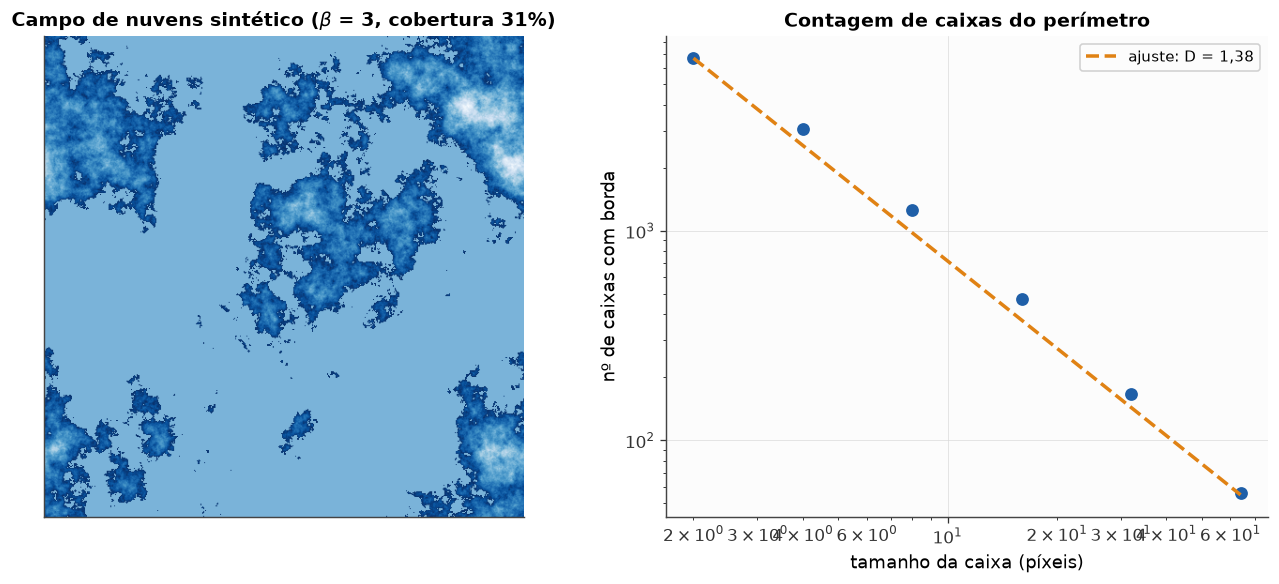
\includegraphics[height=0.5\textheight,width=\linewidth,keepaspectratio]{notebook_fractal.png}\\[-2pt]
    {\tiny campo sintetizado e medido no Caso~3 do notebook do curso}\end{center}
  \end{columns}
\end{frame}

% ---------------------------------------------------------------
\section{Síntese e laboratório}

\begin{frame}{O mapa do capítulo}
  \eqdestaque{UR $\to100\%$: esfriar $|$ subir $|$ misturar \qquad
    $\lambda_{ruas}\simeq3z_i$ \quad $\lambda_{onda}=2\pi U/N$ \quad
    $D\simeq1{,}35$}
  \vspace{0.6em}
  Catálogo (10 gêneros $+$ oktas/teto para o METAR do Cap.~9), três
  caminhos físicos, e os padrões — ruas, ondas, células, fractais — que
  denunciam o mecanismo por baixo.
\end{frame}

\begin{frame}{Laboratório numérico --- notebook do Cap.~6}
  \texttt{notebooks/cap06\_nuvens.ipynb}
  \begin{enumerate}
    \item Diagrama de mistura: bafo e contrails.
    \item EDO do nevoeiro de radiação (formação e conteúdo de água).
    \item Nuvens fractais sintéticas e contagem de caixas.
  \end{enumerate}
  \vspace{0.4em}
  \textbf{Exercícios}: T1--T5 e N1--N4 nas notas; células reservadas no
  notebook.
  \vfill
  \atribuicao
\end{frame}

\end{document}
